\documentclass[12pt,titlepage]{article}
\usepackage[toc,page]{appendix}
\usepackage[linktoc=all]{hyperref}
\usepackage{listings}
\usepackage{graphicx}
\usepackage{xcolor}

% Define style for source code
\lstdefinestyle{cppstyle}{
  belowcaptionskip=1\baselineskip,
  breaklines=true,
  language=C++,
  showstringspaces=false,
  numbers=left,
  basicstyle=\footnotesize\ttfamily,
  keywordstyle=\bfseries\color{green!40!black},
  commentstyle=\itshape\color{purple!40!black},
  identifierstyle=\color{blue},
  stringstyle=\color{orange},
}
\lstset{escapechar=@, style=cppstyle, linewidth=\linewidth}

\begin{document}
\title{ECE 303 Lab Technical Memos}
\author{Nicholas Sica}
\date{October 2, 2020}
\maketitle

\tableofcontents
\newpage

\section{Lab 1}
\subsection{Discussion}
The point of this lab was to introduce us to the Arduino toolkit and allow anyone who is new to the platform
time to adjust and get familiar with the tools presented to them. The lab was straightforward, connect an LED
and resistor to a pin on the arduino and writing simplistic code to change the pulse width modulation values.
The output is as expected, with the intensity of the light changing based off the number put into the serial
monitor, zero being off and 255 being full brightness.
\begin{figure}[!htb]
  \centering
  \includegraphics[width=5.0in]{lab_1/schematic.png}
  \caption{Basic LED Circuit Setup}\label{fig:lab_1}
\end{figure}
\newpage
\section{Lab 2}
\subsection{Discussion}
This lab was used to get us acquainted with timers and learn not only how to set up the correct bit values,
but also how to use them efficiently. A lot of the time was spent debugging the bit values that the different
masks are initialized with as well as learning how to turn the interrupts off efficiently. When run, every
LED blinks at a slow pace and each guess for the code either causes it to blink faster, if wrong, or turn
off, if correct. When the user is out of attempts, the remaining LEDs stay permanently on.
\begin{equation} \label{eq:ocr3a}
  OCR3A = \frac{16\times10^6}{p\times f} - 1
\end{equation}
The value of the register was found using equation~\ref{eq:ocr3a}, where p is the prescalar, in this case
1024, and f is the target frequency, in this case around 0.5 hertz or a 2 second period. Every subsequent
wrong guess, it was divided by two to make it go faster.
\begin{figure}[!htb]
  \centering
  \includegraphics[width=3.25in]{lab_2/schematic.png}
  \caption{Codebreaker Circuit Setup}\label{fig:lab_2}
\end{figure}
\subsection{Hardware}
Figure~\ref{fig:lab_2} shows the setup of the circuit. The setup of the hardware was very similar to
the previous lab, but this time there are four LEDs and care was taken to connect to them to the correct
pin corresponding to the timer we want to use for it.
\newpage
\section{Lab 3}
\subsection{Discussion}
This lab was used to get us to get more comfortable with timers in a different way as well as introduce us
to a photocell. This time around not a lot of time was spent getting the correct timer values, we just
had to make sure that they represented the correct duty cycle. The results for this lab were a bit worse due
to lights coming from my computer. I covered it with a box, but there was bound to be some leakage.
It would have been better if I could isolate my circuit in a container and have my photocell the perfect
distance from the LED. After copying all the data to excel the voltage divider equation shown in 
Equation~\ref{eq:volt_div} was used to get the resistances of the photocell and led.
$V_{DD}$ is the source voltage, in this case 5V, $R_{gnd}$ is the resistor leading to ground, 10k in the
photocell circuit and 1k in the led circuit, $V_{out}$ is the voltage read from pin A0 for the led and pin A1
for the photocell.  
\begin{equation} \label{eq:volt_div}
  R = \frac{V_{DD} \times R_{gnd}}{V_{out}} - R_{gnd}
\end{equation}
\begin{figure}[!htb]
    \centering
    \includegraphics[width=5in]{lab_3/duty_cycle_led_circuit_curr.png}
    \caption{Duty Cycle Versus LED Circuit Current}\label{fig:duty_cycle_led_circuit_curr}
\end{figure}
\begin{figure}[!htb]
    \centering
    \includegraphics[width=5in]{lab_3/duty_cycle_led_res.png}
    \caption{Duty Cycle Versus LED Resistance}\label{fig:duty_cycle_led_res}
\end{figure}
\begin{figure}[!htb]
    \centering
    \includegraphics[width=5in]{lab_3/duty_cycle_photo_curr.png}
    \caption{Duty Cycle Versus Photocell Current}\label{fig:duty_cycle_photo_curr}
\end{figure}
\begin{figure}[!htb]
  \centering
  \includegraphics[width=5in]{lab_3/duty_cycle_photo_res.png}
  \caption{Duty Cycle Versus Photocell Resistance}\label{fig:duty_cycle_photo_res}
\end{figure}
\begin{figure}[!htb]
    \centering
    \includegraphics[width=5in]{lab_3/photo_res_led_curr.png}
    \caption{Photocell Resistance Versus LED Current}\label{fig:photo_res_led_curr}
\end{figure}
The voltage of the LED and photocell were found by using Kirchoff's Voltage law and subtracting the voltage
across the respective resistor from 5V. Lastly, the currents were found using the previous values found for
voltage and resistance and applying Ohm's Law. An error in the values read from pin A0 was introduced due to
the fact that we were reading it from a PWM source. Figure~\ref{fig:duty_cycle_led_circuit_curr} shows the
duty cycle versus LED circuit current which is what you'd expect, a constant value after it gets up and
running. Figure~\ref{fig:duty_cycle_led_res} shows the duty cycle versus the LED resistance which is a
constant value due to the voltage applied not changing. Figure~\ref{fig:duty_cycle_photo_curr}
shows duty cycle versus photocell current which is increasing due to the resistance in the photocell
decreasing as the LED strength increases. Figure~\ref{fig:duty_cycle_photo_res} shows duty cycle versus
photocell resistance which is decreasing due to the LED growing in strength. Finally,
Figure~\ref{fig:photo_res_led_curr} which shows photocell resistance versus LED current which is the most
interesting because it is fairly constant until it suddenly dips.
\subsection{Hardware}
Figure~\ref{fig:lab_3_schem} shows the setup of the circuit. The setup of the hardware was very simple, but
could've been improved with a housing that blocks out light. You could also get different results depending
on the distance the photocell was from the LED, which could lead to skewed results when swapping the LED out
for another color.
\begin{figure}[!htb]
    \centering
    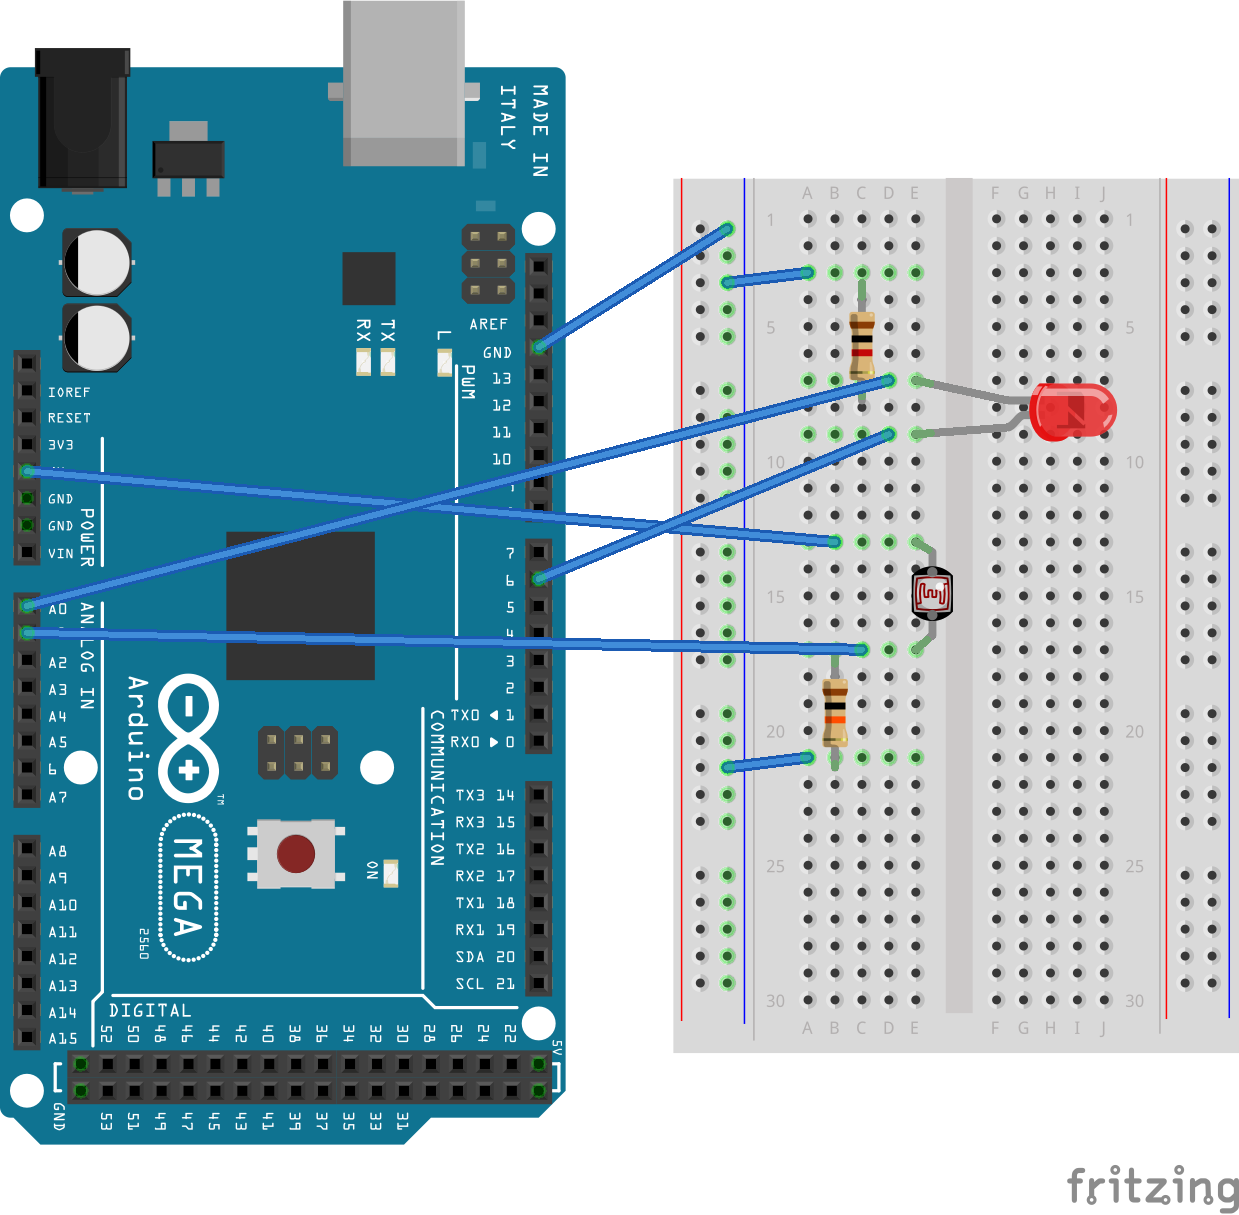
\includegraphics[width=3.25in]{lab_3/schematic.png}
    \caption{Photocell and LED Circuit Setup}\label{fig:lab_3_schem}
\end{figure}
\section{Lab 4}
\subsection{Discussion}
This lab was used to introduce us to using Python or MATLAB in sync with the arduino and teach us how to connect the two and gather data automatically.
This time around not a lot of time was spent getting the correct timer values, we just had to make sure that they represented the correct duty cycle.
The results for this lab, like the last one, were a bit worse due to lights coming from my computer. I covered it with a box, but there was bound to be some leakage.
It would have been better if I could isolate my circuit in a container and have my photocell the perfect distance from the LED. The same basic idea was used as the
last lab except this time there was serial communication through Python and all the graphs were made using matplotlib.
\begin{figure}[!htb]
    \centering
    \includegraphics[width=5in]{lab_4/duty_cycle_led_circuit_curr.png}
    \caption{White Duty Cycle Versus LED Circuit Current}\label{fig:white_lab_4_duty_cycle_led_circuit_curr}
\end{figure}
\begin{figure}[!htb]
    \centering
    \includegraphics[width=5in]{lab_4/duty_cycle_led_res.png}
    \caption{White Duty Cycle Versus LED Resistance}\label{fig:white_lab_4_duty_cycle_led_res}
\end{figure}
\begin{figure}[!htb]
    \centering
    \includegraphics[width=5in]{lab_4/duty_cycle_photo_curr.png}
    \caption{White Duty Cycle Versus Photocell Current}\label{fig:white_lab_4_duty_cycle_photo_curr}
\end{figure}
\begin{figure}[!htb]
  \centering
  \includegraphics[width=5in]{lab_4/duty_cycle_photo_res.png}
  \caption{White Duty Cycle Versus Photocell Resistance}\label{fig:white_lab_4_duty_cycle_photo_res}
\end{figure}
\begin{figure}[!htb]
    \centering
    \includegraphics[width=5in]{lab_4/photo_res_led_curr.png}
    \caption{White Photocell Resistance Versus LED Current}\label{fig:white_lab_4_photo_res_led_curr}
\end{figure}
\begin{figure}[!htb]
  \centering
  \includegraphics[width=5in]{lab_4/duty_cycle_led_circuit_curr.png}
  \caption{Red Duty Cycle Versus LED Circuit Current}
\end{figure}
\begin{figure}[!htb]
  \centering
  \includegraphics[width=5in]{lab_4/duty_cycle_led_res.png}
  \caption{Red Duty Cycle Versus LED Resistance}
\end{figure}
\begin{figure}[!htb]
  \centering
  \includegraphics[width=5in]{lab_4/duty_cycle_photo_curr.png}
  \caption{Red Duty Cycle Versus Photocell Current}
\end{figure}
\begin{figure}[!htb]
\centering
\includegraphics[width=5in]{lab_4/duty_cycle_photo_res.png}
\caption{Red Duty Cycle Versus Photocell Resistance}
\end{figure}
\begin{figure}[!htb]
  \centering
  \includegraphics[width=5in]{lab_4/photo_res_led_curr.png}
  \caption{Red Photocell Resistance Versus LED Current}
\end{figure}
\begin{figure}[!htb]
  \centering
  \includegraphics[width=5in]{lab_4/duty_cycle_led_circuit_curr.png}
  \caption{Yellow Duty Cycle Versus LED Circuit Current}
\end{figure}
\begin{figure}[!htb]
  \centering
  \includegraphics[width=5in]{lab_4/duty_cycle_led_res.png}
  \caption{Yellow Duty Cycle Versus LED Resistance}
\end{figure}
\begin{figure}[!htb]
  \centering
  \includegraphics[width=5in]{lab_4/duty_cycle_photo_curr.png}
  \caption{Yellow Duty Cycle Versus Photocell Current}
\end{figure}
\begin{figure}[!htb]
\centering
\includegraphics[width=5in]{lab_4/duty_cycle_photo_res.png}
\caption{Yellow Duty Cycle Versus Photocell Resistance}
\end{figure}
\begin{figure}[!htb]
  \centering
  \includegraphics[width=5in]{lab_4/photo_res_led_curr.png}
  \caption{Yellow Photocell Resistance Versus LED Current}
\end{figure}
\begin{figure}[!htb]
  \centering
  \includegraphics[width=5in]{lab_4/duty_cycle_led_circuit_curr.png}
  \caption{Blue Duty Cycle Versus LED Circuit Current}
\end{figure}
\begin{figure}[!htb]
  \centering
  \includegraphics[width=5in]{lab_4/duty_cycle_led_res.png}
  \caption{Blue Duty Cycle Versus LED Resistance}
\end{figure}
\begin{figure}[!htb]
  \centering
  \includegraphics[width=5in]{lab_4/duty_cycle_photo_curr.png}
  \caption{Blue Duty Cycle Versus Photocell Current}
\end{figure}
\begin{figure}[!htb]
\centering
\includegraphics[width=5in]{lab_4/duty_cycle_photo_res.png}
\caption{Blue Duty Cycle Versus Photocell Resistance}
\end{figure}
\begin{figure}[!htb]
  \centering
  \includegraphics[width=5in]{lab_4/photo_res_led_curr.png}
  \caption{Blue Photocell Resistance Versus LED Current}
\end{figure}
\begin{figure}[!htb]
  \centering
  \includegraphics[width=5in]{lab_4/duty_cycle_led_circuit_curr.png}
  \caption{Green Duty Cycle Versus LED Circuit Current}
\end{figure}
\begin{figure}[!htb]
  \centering
  \includegraphics[width=5in]{lab_4/duty_cycle_led_res.png}
  \caption{Green Duty Cycle Versus LED Resistance}
\end{figure}
\begin{figure}[!htb]
  \centering
  \includegraphics[width=5in]{lab_4/duty_cycle_photo_curr.png}
  \caption{Green Duty Cycle Versus Photocell Current}
\end{figure}
\begin{figure}[!htb]
\centering
\includegraphics[width=5in]{lab_4/duty_cycle_photo_res.png}
\caption{Green Duty Cycle Versus Photocell Resistance}
\end{figure}
\begin{figure}[!htb]
  \centering
  \includegraphics[width=5in]{lab_4/photo_res_led_curr.png}
  \caption{Green Photocell Resistance Versus LED Current}
\end{figure}
The values of the voltage, current, and resistance were found using the same method as the last lab. An error in the values read from pin A0 was introduced due to
the fact that we were reading it from a PWM source. Figure~\ref{fig:white_lab_4_duty_cycle_led_circuit_curr} shows the
duty cycle versus LED circuit current. You are seeing a finer grain look than last time and even get to see a bit of the PWM in action. Figure~\ref{fig:white_lab_4_duty_cycle_led_res}
shows the duty cycle versus the LED resistance which is a constant value due to the voltage applied not changing. Figure~\ref{fig:white_lab_4_duty_cycle_photo_curr}
shows duty cycle versus photocell current which is increasing due to the resistance in the photocell decreasing as the LED strength increases. The part at the end where it dips
is probably due to the imperfect setup we have and finer granularity than the excel version. Figure~\ref{fig:white_lab_4_duty_cycle_photo_res} shows duty cycle versus photocell
resistance which is decreasing due to the LED growing in strength. It starting at zero could also be due to the imperfect setup or the photoreistor not picking up the light at a
low strength. Finally, Figure~\ref{fig:white_lab_4_photo_res_led_curr} which shows photocell resistance versus LED current which is different than last time due to the fact that
the LED current isn't constant because of the decreased step size causing it to be jumpier.
\subsection{Hardware}
Figure~\ref{fig:lab_3_schem} shows the setup of the circuit. The setup of the hardware was very simple, but
could've been improved with a housing that blocks out light. You could also get different results depending
on the distance the photocell was from the LED, which could lead to skewed results when swapping the LED out
for another color.
\clearpage
\begin{appendices}
  \section{Program Code}
  \subsection{Lab 1 Code}
  \begin{minipage}{\linewidth}
    \lstinputlisting[caption={Lab 1 Arduino Code- Blinky}, captionpos=b, label={lst:lab_1_blinky}, language=C++]{../lab_1/src/blinky.cpp}
  \end{minipage} 
  \begin{minipage}{\linewidth}
    \lstinputlisting[caption={Lab 1 Arduino Code- Variable Brightness}, captionpos=b, label={lst:lab_1_variable}, language=C++]{../lab_1/src/main.cpp}
  \end{minipage} 
  \subsection{Lab 2 Code}
    \lstinputlisting[caption={Lab 2 Arduino Code}, captionpos=b label={lst:lab_2}, language=C++]{../lab_2/src/main.cpp}
  \subsection{Lab 3 Code}
    \lstinputlisting[caption={Lab 3 Arduino Code}, captionpos=b label={lst:lab_3}, language=C++]{../lab_3/src/main.cpp}
  \subsection{Lab 4 Code}
    \lstinputlisting[caption={Lab 4 Arduino Code}, captionpos=b label={lst:lab_4_arduino}, language=C++]{../lab_4/src/main.cpp}
    \lstinputlisting[caption={Lab 4 Python Code}, captionpos=b label={lst:lab_4_python}, language=Python]{../lab_4/src/frontend.py}
\end{appendices}
\end{document}
%%% Local Variables:
%%% mode: latex
%%% TeX-master: t
%%% End:
